\documentclass{beamer}
\mode <presentation>
{
    \usetheme{PaloAlto}
    \usecolortheme{seagull}
    \setbeamercovered{transparent}
}

\usepackage[english]{babel}
\usepackage{times}
\usepackage{amsmath}
% math extension - one probably wants to use symbols like '[' (written as '$[$')
\usepackage{ucs}
%\usepackage[utf8]{inputenc}
\usepackage[utf8x]{inputenc}

%\setbeamercolor{background canvas}{bg=
\includegraphics[width=\textwidth]{./pics/wolf.png}}

\title{Assets management with~FusionInventory~and~GLPI}
\subject{Assets management with FusionInventory and GLPI}
\keywords{Assets management, Inventory, FusionInventory, GLPI}

\date{
\includegraphics[height=0.3cm]{./pics/cc-by-sa.png} ~ 6th February, 2011}
\titlegraphic{}
\subtitle{
\includegraphics[width=0.9\linewidth]{./pics/wolf.png}}
\institute{
\includegraphics[height=1.2cm]{./pics/esquimaux-logo.png}}
\author{ FusionInventory project }
\logo{
\includegraphics[height=1cm]{./pics/esquimaux-logo.png}}

%\setcounter{tocdepth}{1}

\AtBeginSubsection[] % Do nothing for \subsection*
{
    \begin{frame}<beamer>
        \frametitle{Outline}
    % Only list the subsection of the current section
        \addtocontents{toc}{\protect\setcounter{tocdepth}{2}}
    % http://tex.stackexchange.com/questions/4102/setting-setcountertocdepth-for-an-individual-chapter
        \tableofcontents[currentsection,currentsubsection]
        \end{frame}
}

\AtBeginSection[] % Do nothing for \section*
{
    \begin{frame}<beamer>
        \frametitle{Outline}
    % Only list the section
        \addtocontents{toc}{\protect\setcounter{tocdepth}{1}}
    \tableofcontents[currentsection]
        \end{frame}
}


\begin{document}

\frame[plain]{\titlepage}

%\begin{frame}
% \frametitle{Outline}
% \tableofcontents
%\end{frame}

\author{\href{http://www.FusionInventory.org}{FusionInventory.org}}

\tableofcontents[pausesections]

\section{Overview}

\begin{frame}
\frametitle{Global overview}

\begin{itemize}
%
\item here a schema
%
\end{itemize}
\end{frame}


\section{Agent}

%
\subsection{Agent history}
%-------------------------------------------------------------------
\begin{frame}
\frametitle{Agent history}

\begin{itemize}
%
\item todo
%
\end{itemize}
\end{frame}
%-------------------------------------------------------------------
\subsection{the internal}
%-------------------------------------------------------------------
\begin{frame}
\frametitle{The agent internal}
%
\begin{itemize}
%
\item todo 
%
\end{itemize}
\end{frame}

\subsection{task}
%-------------------------------------------------------------------
\begin{frame}
\frametitle{Task}
%
\begin{itemize}
%
\item todo 
%
\end{itemize}
\end{frame}



\subsection{supported OS}
%-------------------------------------------------------------------
\begin{frame}
\frametitle{supported OS}
%
\begin{itemize}
%
\item todo 
%
\end{itemize}
\end{frame}

%-------------------------------------------------------------------
\section{The server side: FusionInventory for GLPI}
%
\logo{
\includegraphics[height=1cm]{./pics/fusioninventory-logo.png}}
%
\subsection{History}
%-------------------------------------------------------------------
\begin{frame}
\frametitle{A long long time ago}
%
\begin{itemize}
\item Tracker 
%
\end{itemize}
\end{frame}

\subsection{Internal}
%-------------------------------------------------------------------
\begin{frame}
\frametitle{GLPI plugin}
%
\begin{itemize}
\item FusionInventory for GLPI is ... a plugin for ... GLPI. Wait! What? 
%
\end{itemize}
\end{frame}

%-------------------------------------------------------------------
\begin{frame}
\frametitle{GLPI plugin}
%
\begin{itemize}
\item PHP/MySQL
%
\end{itemize}
\end{frame}

\subsection{Data exchange}
%-------------------------------------------------------------------
\begin{frame}
\frametitle{the protocol}
%
\begin{itemize}
\item HTTPS everywhere! 
%
\end{itemize}
\end{frame}



%-------------------------------------------------------------------
\section{What can I do with that?}
%-------------------------------------------------------------------
%-------------------------------------------------------------------
\subsection{first, machine Inventory!}
%-------------------------------------------------------------------
\begin{frame}
\frametitle{The inventories}

\begin{itemize}
%
\item local - hardware including USB devices, screens
%
\end{itemize}
\end{frame}
%-------------------------------------------------------------------
\subsection{network discovery!}
%-------------------------------------------------------------------

\logo{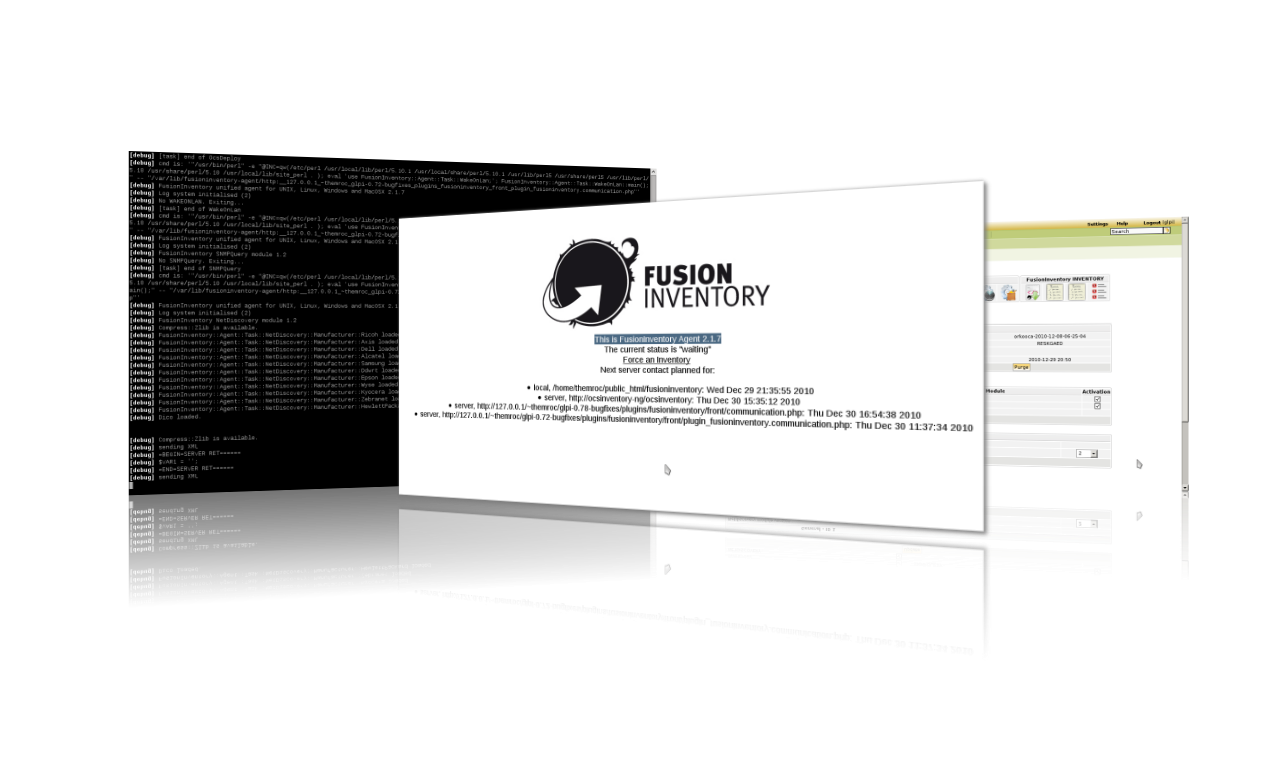
\includegraphics[height=4cm]{./pics/fusioninventory-tasks.png}}

\begin{frame}
\frametitle{Identify devices on the network}
%
\begin{itemize}
%
\item TODO
%
\end{itemize}
\end{frame}
%-------------------------------------------------------------------
\subsection{switch inventory}
%-------------------------------------------------------------------
\logo{
\includegraphics[height=1cm]{./pics/fusioninventory-logo.png}}

\begin{frame}
\frametitle{Switch inventory}

\begin{itemize}
%
\item TODO
%
\end{itemize}
\end{frame}
%-------------------------------------------------------------------
\subsection{printer status}
%-------------------------------------------------------------------

\logo{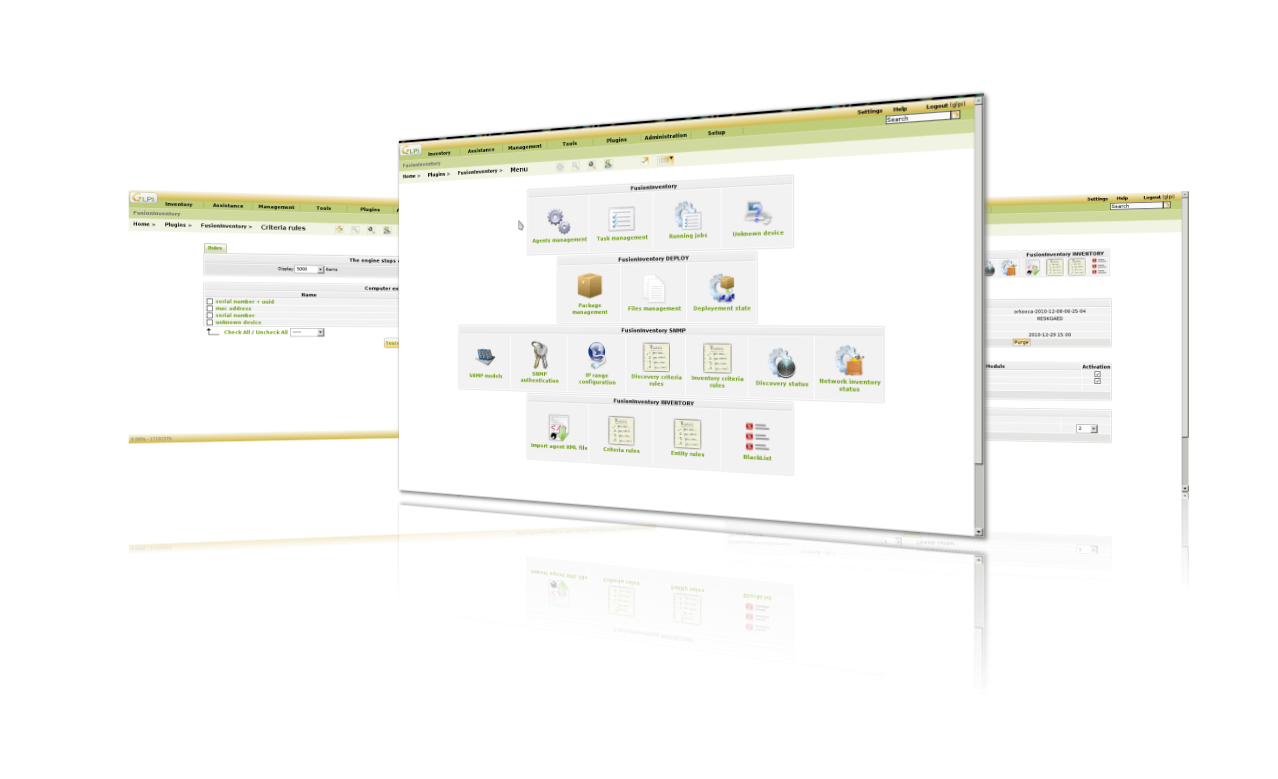
\includegraphics[height=3.5cm]{./pics/fusioninventory-glpi.png}}

\begin{frame}
\frametitle{printer too!}

\begin{itemize}

\item TODO

\end{itemize}
\end{frame}
%-------------------------------------------------------------------
\subsection{Wake on LAN}
%-------------------------------------------------------------------
\begin{frame}
\frametitle{Wake on LAN}
\logo{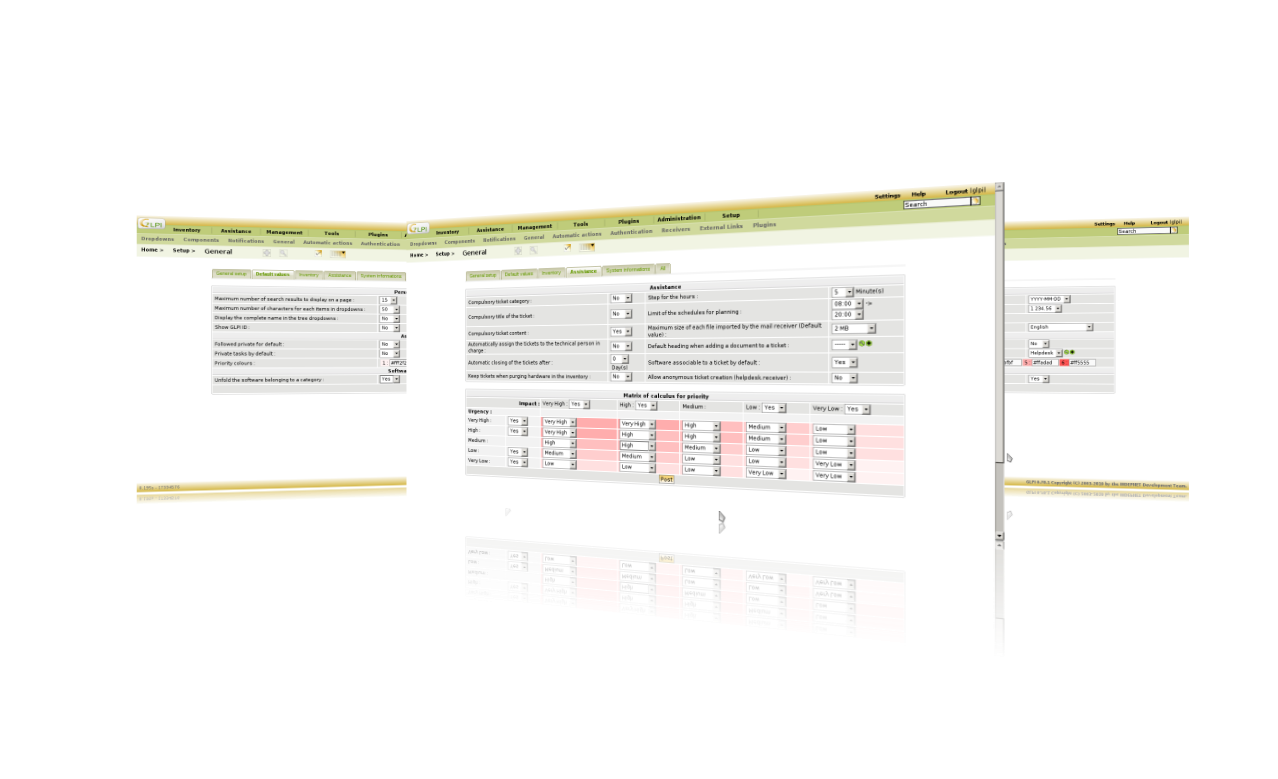
\includegraphics[height=3.5cm]{./pics/glpi-config.png}}
\begin{itemize}
%
\item TODO
%
\end{itemize}
\end{frame}

%-------------------------------------------------------------------
\subsection{Software deployment}
%-------------------------------------------------------------------
\logo{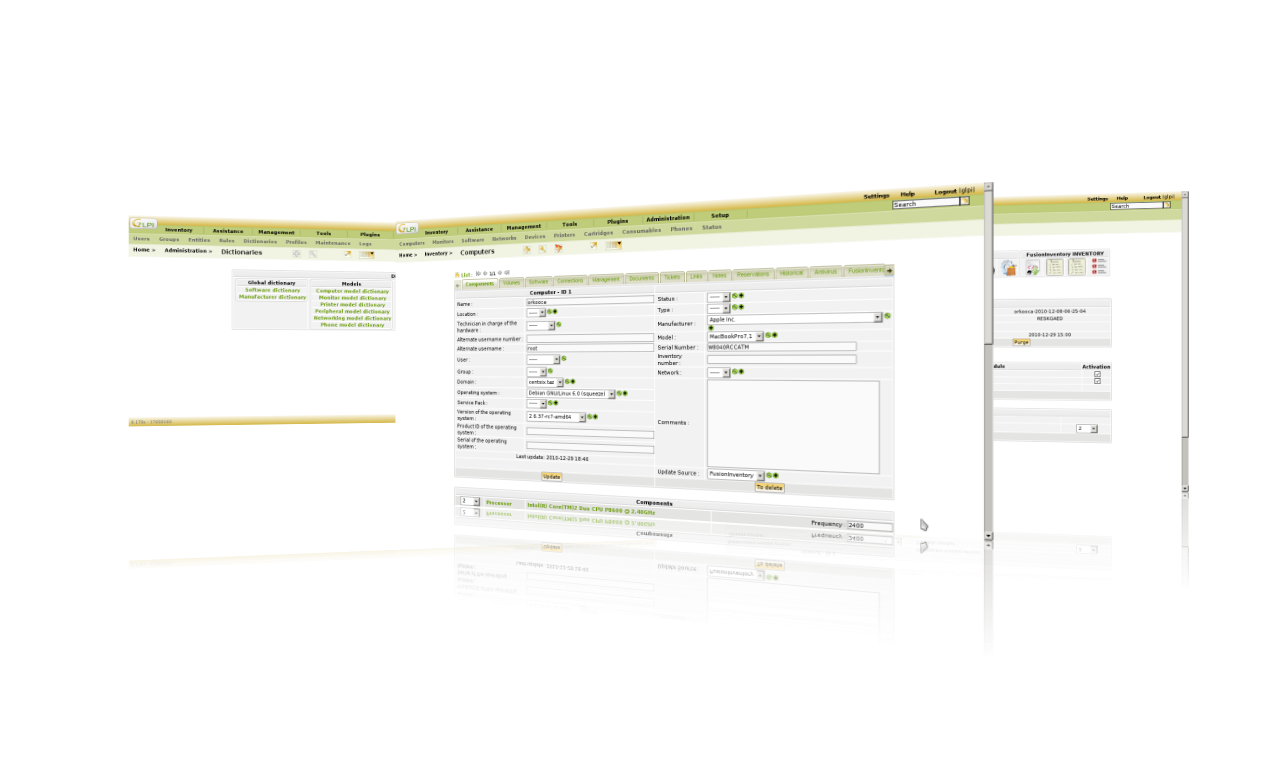
\includegraphics[height=3.5cm]{./pics/glpi-inventory.png}}

\begin{frame}
\frametitle{Software deployment}

\begin{itemize}
%
\item TODO
%
\end{itemize}
\end{frame}
%-------------------------------------------------------------------
\subsection{Task Scheduling}
%-------------------------------------------------------------------
\logo{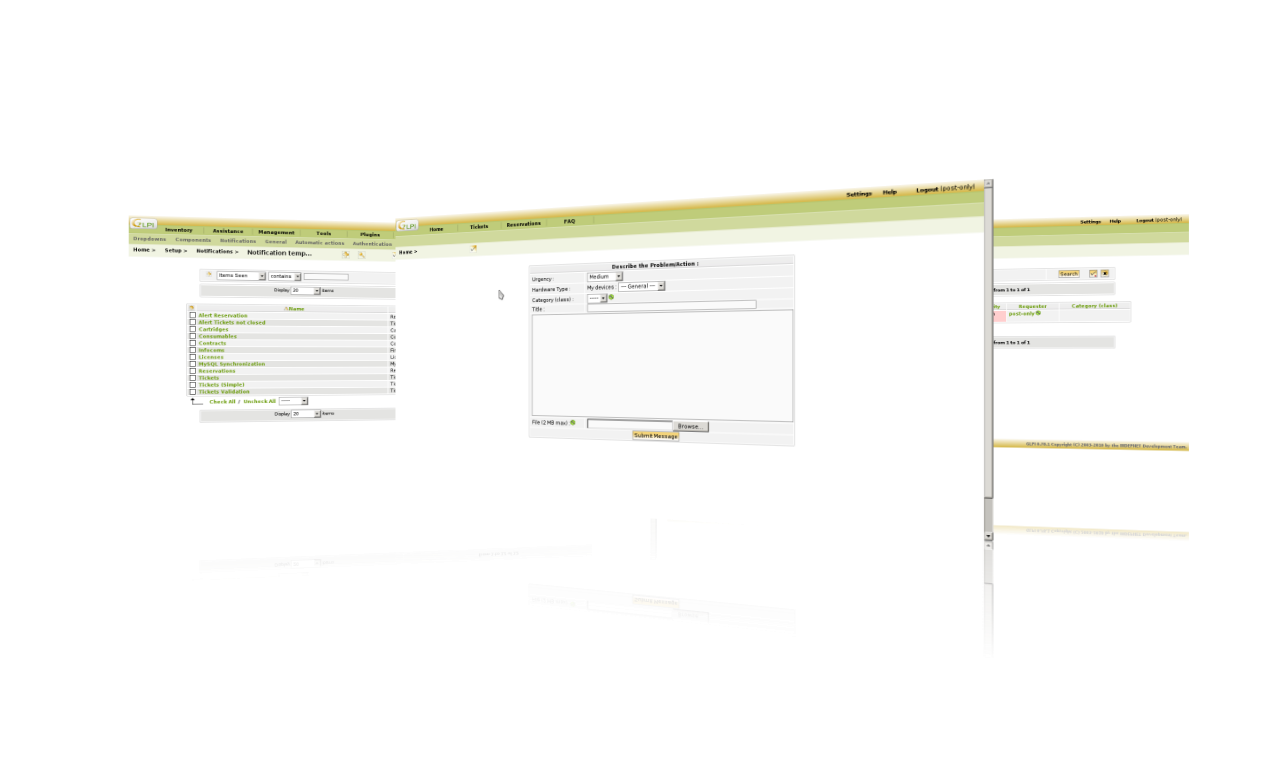
\includegraphics[height=3.5cm]{./pics/glpi-helpdesk.png}}
\begin{frame}
\frametitle{Task Scheduling}
%
\begin{itemize}
%
\item TODO
%
\end{itemize}
\end{frame}
%-------------------------------------------------------------------
\subsection{libFusionInventory}
%-------------------------------------------------------------------
\logo{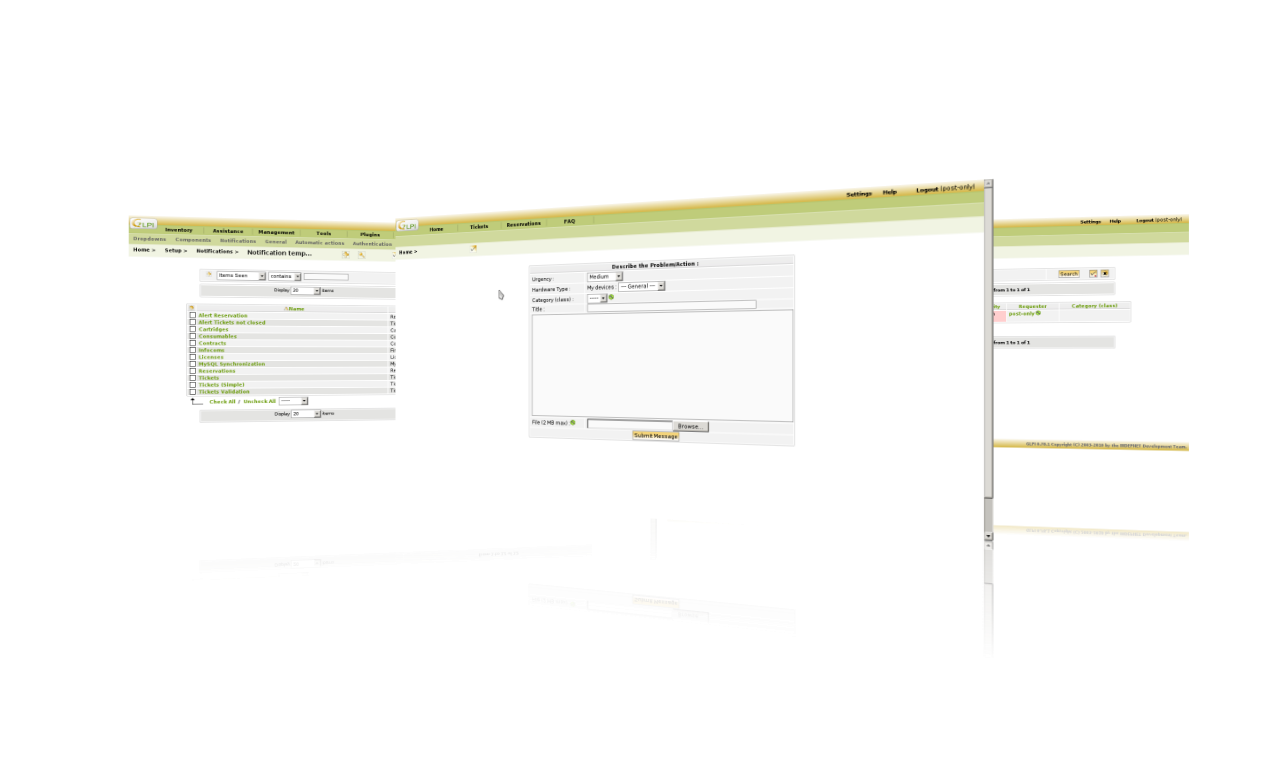
\includegraphics[height=3.5cm]{./pics/glpi-helpdesk.png}}
\begin{frame}
\frametitle{libFusionInventory}
%
\begin{itemize}
%
\item TODO
%
\end{itemize}
\end{frame}
%

%-------------------------------------------------------------------
\section{Roadmap}
%-------------------------------------------------------------------
\logo{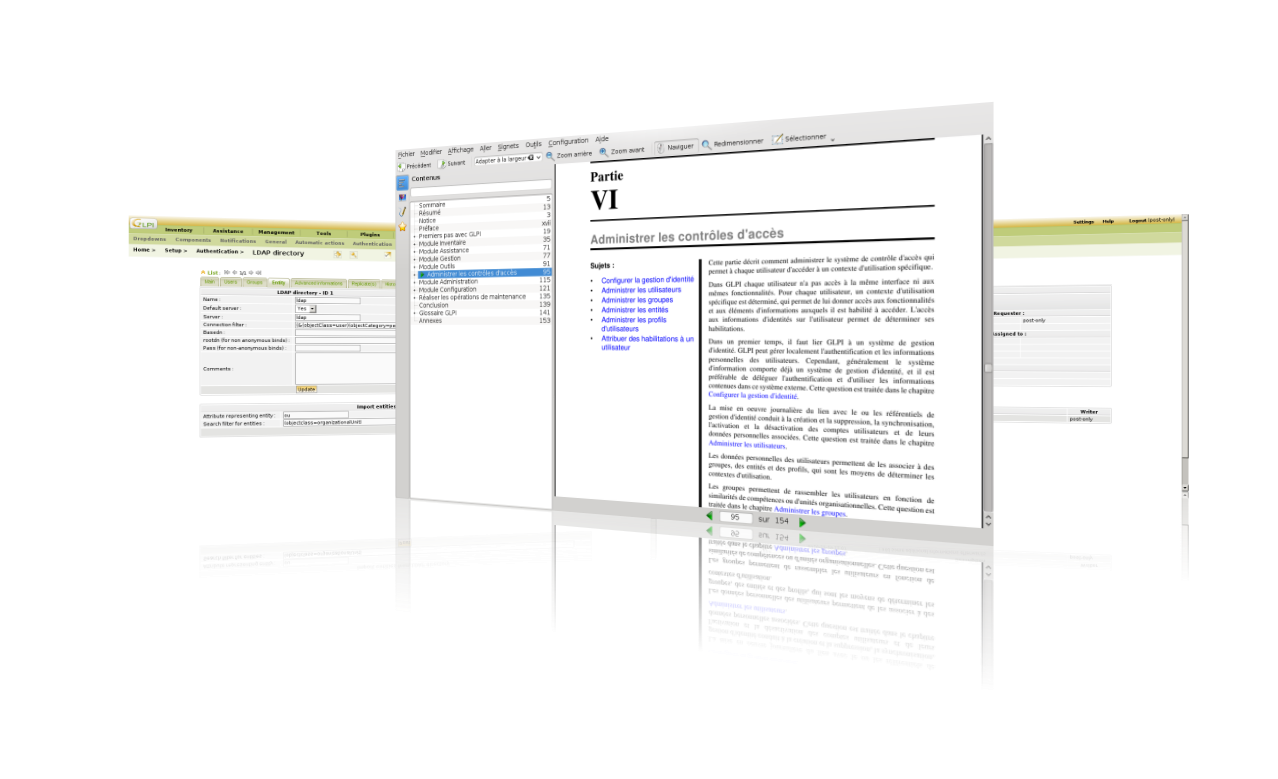
\includegraphics[height=3.5cm]{./pics/glpi-doc.png}}
%
\begin{frame}
\frametitle{Our roadmap}
%
\begin{itemize}
%
\item TODO
%
\end{itemize}
\end{frame}

\section{Community}
%-------------------------------------------------------------------
\logo{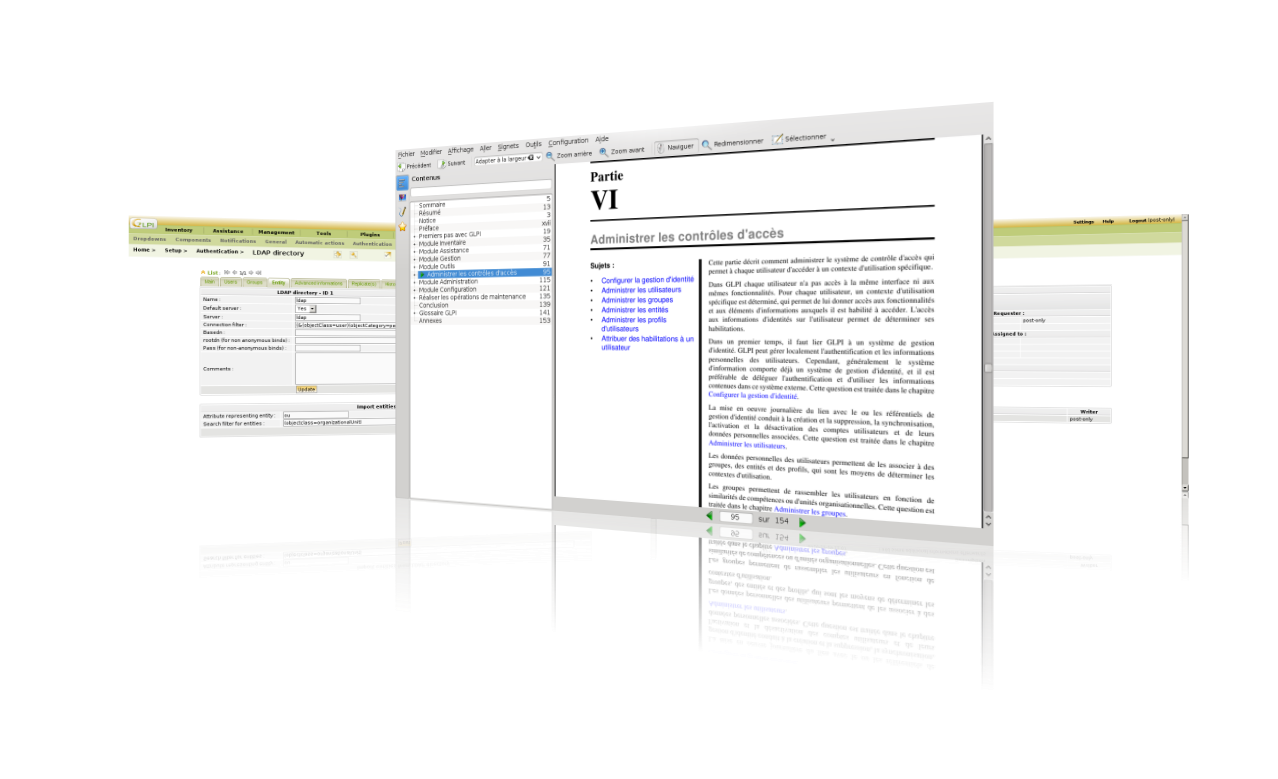
\includegraphics[height=3.5cm]{./pics/glpi-doc.png}}
%
\begin{frame}
\frametitle{Our roadmap}
%
\begin{itemize}
%
\item TODO
%
\end{itemize}
\end{frame}

\section{Question?}
%-------------------------------------------------------------------
\logo{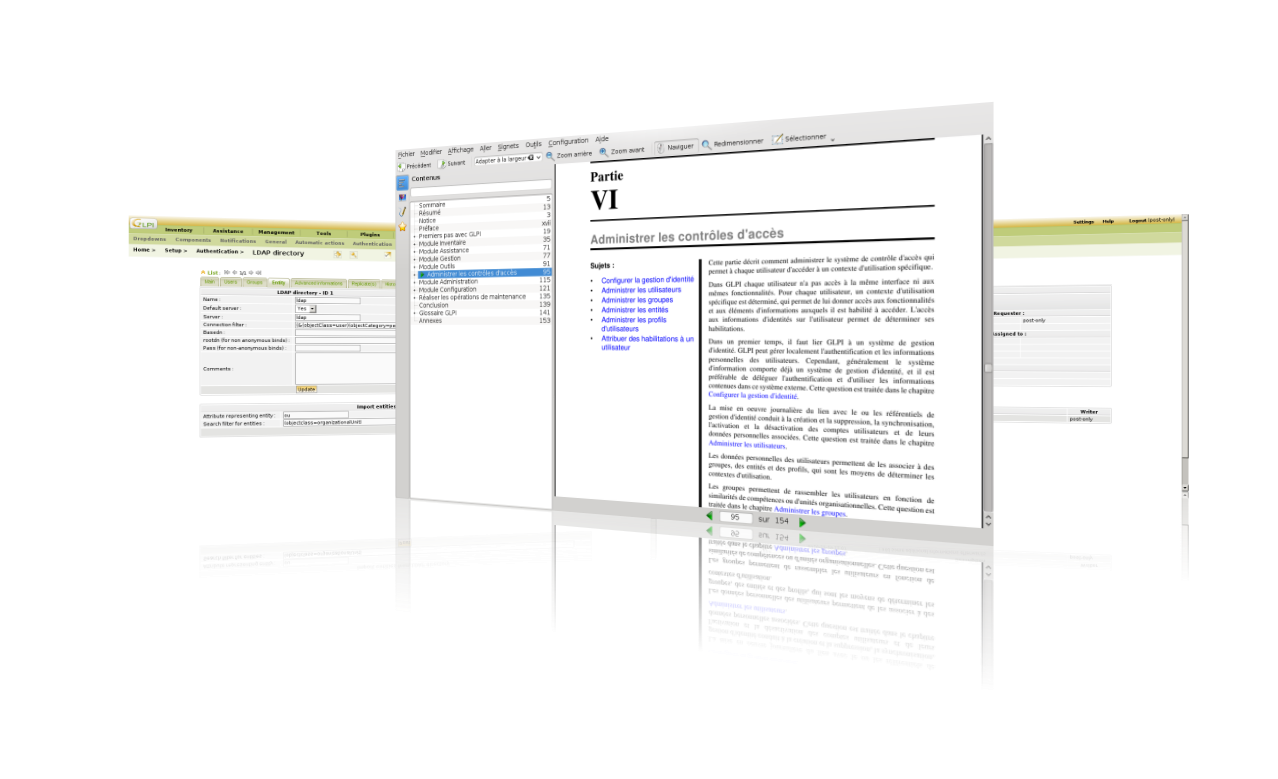
\includegraphics[height=3.5cm]{./pics/glpi-doc.png}}
%
\begin{frame}
\frametitle{Question?}
%
\begin{itemize}
%
\item TODO
%
\end{itemize}
\end{frame}

\logo{
\includegraphics[height=1.5cm]{./pics/esquimaux-logo.png}}

\setbeamertemplate{headline}{
\includegraphics[width=\paperwidth, height=2cm, clip=true]{./pics/header.png}}
%\begin{frame}[plain]
\begin{frame}[shrink=20]{Outline}

\tableofcontents
%
\includegraphics[width=\columnwidth]{./pics/wolf.png} 
%\\
        %
\includegraphics[height=1.5cm]{./pics/esquimaux-logo.png}

        \end{frame}
        \end{document}
